\documentclass[preprint, 3p,
authoryear]{elsarticle} %review=doublespace preprint=single 5p=2 column
%%% Begin My package additions %%%%%%%%%%%%%%%%%%%

\usepackage[hyphens]{url}

  \journal{An awesome journal} % Sets Journal name

\usepackage{graphicx}
%%%%%%%%%%%%%%%% end my additions to header

\usepackage[T1]{fontenc}
\usepackage{lmodern}
\usepackage{amssymb,amsmath}
% TODO: Currently lineno needs to be loaded after amsmath because of conflict
% https://github.com/latex-lineno/lineno/issues/5
\usepackage{lineno} % add
\usepackage{ifxetex,ifluatex}
\usepackage{fixltx2e} % provides \textsubscript
% use upquote if available, for straight quotes in verbatim environments
\IfFileExists{upquote.sty}{\usepackage{upquote}}{}
\ifnum 0\ifxetex 1\fi\ifluatex 1\fi=0 % if pdftex
  \usepackage[utf8]{inputenc}
\else % if luatex or xelatex
  \usepackage{fontspec}
  \ifxetex
    \usepackage{xltxtra,xunicode}
  \fi
  \defaultfontfeatures{Mapping=tex-text,Scale=MatchLowercase}
  \newcommand{\euro}{€}
\fi
% use microtype if available
\IfFileExists{microtype.sty}{\usepackage{microtype}}{}
\usepackage[]{natbib}
\bibliographystyle{plainnat}

\ifxetex
  \usepackage[setpagesize=false, % page size defined by xetex
              unicode=false, % unicode breaks when used with xetex
              xetex]{hyperref}
\else
  \usepackage[unicode=true]{hyperref}
\fi
\hypersetup{breaklinks=true,
            bookmarks=true,
            pdfauthor={},
            pdftitle={Short Paper},
            colorlinks=false,
            urlcolor=blue,
            linkcolor=magenta,
            pdfborder={0 0 0}}

\setcounter{secnumdepth}{5}
% Pandoc toggle for numbering sections (defaults to be off)

% Pandoc syntax highlighting
\usepackage{color}
\usepackage{fancyvrb}
\newcommand{\VerbBar}{|}
\newcommand{\VERB}{\Verb[commandchars=\\\{\}]}
\DefineVerbatimEnvironment{Highlighting}{Verbatim}{commandchars=\\\{\}}
% Add ',fontsize=\small' for more characters per line
\usepackage{framed}
\definecolor{shadecolor}{RGB}{248,248,248}
\newenvironment{Shaded}{\begin{snugshade}}{\end{snugshade}}
\newcommand{\AlertTok}[1]{\textcolor[rgb]{0.94,0.16,0.16}{#1}}
\newcommand{\AnnotationTok}[1]{\textcolor[rgb]{0.56,0.35,0.01}{\textbf{\textit{#1}}}}
\newcommand{\AttributeTok}[1]{\textcolor[rgb]{0.13,0.29,0.53}{#1}}
\newcommand{\BaseNTok}[1]{\textcolor[rgb]{0.00,0.00,0.81}{#1}}
\newcommand{\BuiltInTok}[1]{#1}
\newcommand{\CharTok}[1]{\textcolor[rgb]{0.31,0.60,0.02}{#1}}
\newcommand{\CommentTok}[1]{\textcolor[rgb]{0.56,0.35,0.01}{\textit{#1}}}
\newcommand{\CommentVarTok}[1]{\textcolor[rgb]{0.56,0.35,0.01}{\textbf{\textit{#1}}}}
\newcommand{\ConstantTok}[1]{\textcolor[rgb]{0.56,0.35,0.01}{#1}}
\newcommand{\ControlFlowTok}[1]{\textcolor[rgb]{0.13,0.29,0.53}{\textbf{#1}}}
\newcommand{\DataTypeTok}[1]{\textcolor[rgb]{0.13,0.29,0.53}{#1}}
\newcommand{\DecValTok}[1]{\textcolor[rgb]{0.00,0.00,0.81}{#1}}
\newcommand{\DocumentationTok}[1]{\textcolor[rgb]{0.56,0.35,0.01}{\textbf{\textit{#1}}}}
\newcommand{\ErrorTok}[1]{\textcolor[rgb]{0.64,0.00,0.00}{\textbf{#1}}}
\newcommand{\ExtensionTok}[1]{#1}
\newcommand{\FloatTok}[1]{\textcolor[rgb]{0.00,0.00,0.81}{#1}}
\newcommand{\FunctionTok}[1]{\textcolor[rgb]{0.13,0.29,0.53}{\textbf{#1}}}
\newcommand{\ImportTok}[1]{#1}
\newcommand{\InformationTok}[1]{\textcolor[rgb]{0.56,0.35,0.01}{\textbf{\textit{#1}}}}
\newcommand{\KeywordTok}[1]{\textcolor[rgb]{0.13,0.29,0.53}{\textbf{#1}}}
\newcommand{\NormalTok}[1]{#1}
\newcommand{\OperatorTok}[1]{\textcolor[rgb]{0.81,0.36,0.00}{\textbf{#1}}}
\newcommand{\OtherTok}[1]{\textcolor[rgb]{0.56,0.35,0.01}{#1}}
\newcommand{\PreprocessorTok}[1]{\textcolor[rgb]{0.56,0.35,0.01}{\textit{#1}}}
\newcommand{\RegionMarkerTok}[1]{#1}
\newcommand{\SpecialCharTok}[1]{\textcolor[rgb]{0.81,0.36,0.00}{\textbf{#1}}}
\newcommand{\SpecialStringTok}[1]{\textcolor[rgb]{0.31,0.60,0.02}{#1}}
\newcommand{\StringTok}[1]{\textcolor[rgb]{0.31,0.60,0.02}{#1}}
\newcommand{\VariableTok}[1]{\textcolor[rgb]{0.00,0.00,0.00}{#1}}
\newcommand{\VerbatimStringTok}[1]{\textcolor[rgb]{0.31,0.60,0.02}{#1}}
\newcommand{\WarningTok}[1]{\textcolor[rgb]{0.56,0.35,0.01}{\textbf{\textit{#1}}}}

% tightlist command for lists without linebreak
\providecommand{\tightlist}{%
  \setlength{\itemsep}{0pt}\setlength{\parskip}{0pt}}

% From pandoc table feature
\usepackage{longtable,booktabs,array}
\usepackage{calc} % for calculating minipage widths
% Correct order of tables after \paragraph or \subparagraph
\usepackage{etoolbox}
\makeatletter
\patchcmd\longtable{\par}{\if@noskipsec\mbox{}\fi\par}{}{}
\makeatother
% Allow footnotes in longtable head/foot
\IfFileExists{footnotehyper.sty}{\usepackage{footnotehyper}}{\usepackage{footnote}}
\makesavenoteenv{longtable}






\begin{document}


\begin{frontmatter}

  \title{Short Paper}
    \author[Some Institute of Technology]{Irina Vélez%
  \corref{cor1}%
  \fnref{1}}
   \ead{alice@example.com} 
    \author[Another University]{Otto Palkama%
  %
  \fnref{1}}
   \ead{bob@example.com} 
      \affiliation[Some Institute of Technology]{
    organization={Big Wig University},addressline={1 main
street},city={Gotham},postcode={123456},state={State},country={United
States},}
    \affiliation[Another University]{
    organization={Department},addressline={A street
29},city={Manchester,},postcode={2054 NX},country={The Netherlands},}
    \cortext[cor1]{Corresponding author}
    \fntext[1]{This is the first author footnote.}
    \fntext[2]{Another author footnote.}
  
  \begin{abstract}
  This is the abstract.

  It consists of two paragraphs.
  \end{abstract}
    \begin{keyword}
    keyword1 \sep 
    keyword2
  \end{keyword}
  
 \end{frontmatter}

\hypertarget{introduction}{%
\section{Introduction}\label{introduction}}

The idea is to explore how the use of Large Language Models (LLMs) as
General Purpose Technology (GPT) could reshape industries, considering
the generalization capabilities of LLMs and the rapid adoption of these
tools by the public and firms.

A. Background on the potential economic impact of Large Language Models
(LLMs) as General Purpose Technology (GPT) B. Objective of the paper:
Exploring how the use of LLMs as GPT could reshape industries and
contribute to economic growth

Generalization of tools seems to be an important characteristic to
leverage the potential of growth and development, because if a same tool
could be broad use for different purposes, so the tool becomes in a very
valuable tool.

Until now the abilities reached by the Large Languages Models LLMs have
arisen to a certain level of computational power that might require
scaling up past this threshold (10\^{}23 training FLOPs), meaning that
they are able to perform multiple tasks related to Text Understanding
and Generation,Problem Solving and Mathematics, Image and Data
Classification, Text Analysis and Comprehension, and so on, but as
\citep{weiemergent} suggested for future works, it could be possible new
abilities could emerge scaling up the models and understanding how
emergence occurs would provide new insights into how to train
more-capable language models.

On the other hand, the use of LLMs as a base technology of other tools,
such as software-AI powered, open a new window and enveloped the
potential of productivity improvements of the work-human force or human
capital as it was mention by \citep{gptaregpts} telling that LLMs such
as GPTs exhibit traits of general-purpose technologies, could have
considerable economic, social, and policy implications.

So, the potential arising of emergent abilities and the wide use of LLMs
as enablers of new tools (AI based-software) alongside the spread use of
tools such as ChatGPT by a large amount of humans (here: million of
users of chatGPT), it could signify a future unseen before by the human
beings, because the expansion and pushing of new boarders and limits
would be accelerated.

\hypertarget{assessing-the-potential-economic-impact}{%
\section{Assessing the Potential Economic
Impact}\label{assessing-the-potential-economic-impact}}

Starting Point - Assessing the potential economic impact of LLMs based
on a retrospective approach: Considering the potential of the AI as a
new GPT, what would be its impact on reshaping industries and economic
growth, base on the behavior of last General Purpose Technology like
internet, electricity, etc.

A. Defining General Purpose Technology (GPT)

General Purpose Technology is a transformative technology with a strong
improvement process at the begining and eventually becoming widely
adopted for its multiples uses, while producing many spillover effects
\citep{paradox}. As such, it have a pervasive impact on society as a
whole, mainly due to its capability to redefine the ways in which
businesses operate, improve productive and contribute to long-term
economic growth. Some well-know examples are steam power, electricity,
semiconductors, and internet.

The positive expectations regarding how new technologies could drive
development, economic growth, and generate substantial profits are often
accompanied by the optimistic mindset of industrial and well-known
technology leaders, as well as venture capitalists. Simultaneously, the
financial sector capitalizes on this excitement through speculative
investments and forecasts of future company wealth. As mentioned by
\citep{paradox}, ``there is no inherent inconsistency between
forward-looking technological optimism and backward-looking
disappointment. Both can simultaneously exist,'' especially during
periods of transformative changes.

B. Evaluating the potential economic impact in terms of value creation
and cost optimization 1. Real cases of successful implementations of
LLMs for value creation 2. Real cases of successful implementations of
LLMs for cost optimization C. Intangible capital - capital may not be
reflected in the measurements of economic growth

\hypertarget{generalization-capabilities-of-llms-as-gpt}{%
\section{Generalization Capabilities of LLMs as
GPT}\label{generalization-capabilities-of-llms-as-gpt}}

A. Examining the adoption rate of previous GPTs B. Key factors
contributing to the widespread adoption of a technology as a GPT C.
Reviewing the literature on the potential of AI as a GPT

\hypertarget{llms-vs.-artificial-general-intelligence-agi}{%
\section{LLMs vs.~Artificial General Intelligence
(AGI)}\label{llms-vs.-artificial-general-intelligence-agi}}

A. Understanding the difference between LLMs and AGI B. Exploring
whether AGI is the real General Purpose Technology

\hypertarget{acknowledging-benefits-and-limitations-of-llms-as-gpt}{%
\section{Acknowledging Benefits and Limitations of LLMs as
GPT}\label{acknowledging-benefits-and-limitations-of-llms-as-gpt}}

A. Discussing the potential benefits of LLMs as GPT B. Addressing the
limitations and challenges associated with LLMs as GPT

\hypertarget{conclusion}{%
\section{Conclusion}\label{conclusion}}

A. Summarizing the main points discussed in the paper B. Emphasizing the
potential of LLMs as GPT in reshaping industries

\hypertarget{bibliography-styles}{%
\section{Bibliography styles}\label{bibliography-styles}}

Here are two sample references: \citeauthor{Feynman1963118}
\citetext{\citeyear{Feynman1963118}; \citealp{Dirac1953888}}.

By default, natbib will be used with the \texttt{authoryear} style, set
in \texttt{classoption} variable in YAML. You can sets extra options
with \texttt{natbiboptions} variable in YAML header. Example

\begin{Shaded}
\begin{Highlighting}[]
\FunctionTok{natbiboptions}\KeywordTok{:}\AttributeTok{ longnamesfirst,angle,semicolon}
\end{Highlighting}
\end{Shaded}

There are various more specific bibliography styles available at
\url{https://support.stmdocs.in/wiki/index.php?title=Model-wise_bibliographic_style_files}.
To use one of these, add it in the header using, for example,
\texttt{biblio-style:\ model1-num-names}.

\hypertarget{using-csl}{%
\subsection{Using CSL}\label{using-csl}}

If \texttt{citation\_package} is set to \texttt{default} in
\texttt{elsevier\_article()}, then pandoc is used for citations instead
of \texttt{natbib}. In this case, the \texttt{csl} option is used to
format the references. Alternative \texttt{csl} files are available from
\url{https://www.zotero.org/styles?q=elsevier}. These can be downloaded
and stored locally, or the url can be used as in the example header.

\hypertarget{equations}{%
\section{Equations}\label{equations}}

Here is an equation: \[ 
  f_{X}(x) = \left(\frac{\alpha}{\beta}\right)
  \left(\frac{x}{\beta}\right)^{\alpha-1}
  e^{-\left(\frac{x}{\beta}\right)^{\alpha}}; 
  \alpha,\beta,x > 0 .
\]

Here is another: \begin{align}
  a^2+b^2=c^2.
\end{align}

Inline equations: \(\sum_{i = 2}^\infty\{\alpha_i^\beta\}\)

\hypertarget{figures-and-tables}{%
\section{Figures and tables}\label{figures-and-tables}}

Figure \ref{fig2} is generated using an R chunk.

\begin{figure}

{\centering 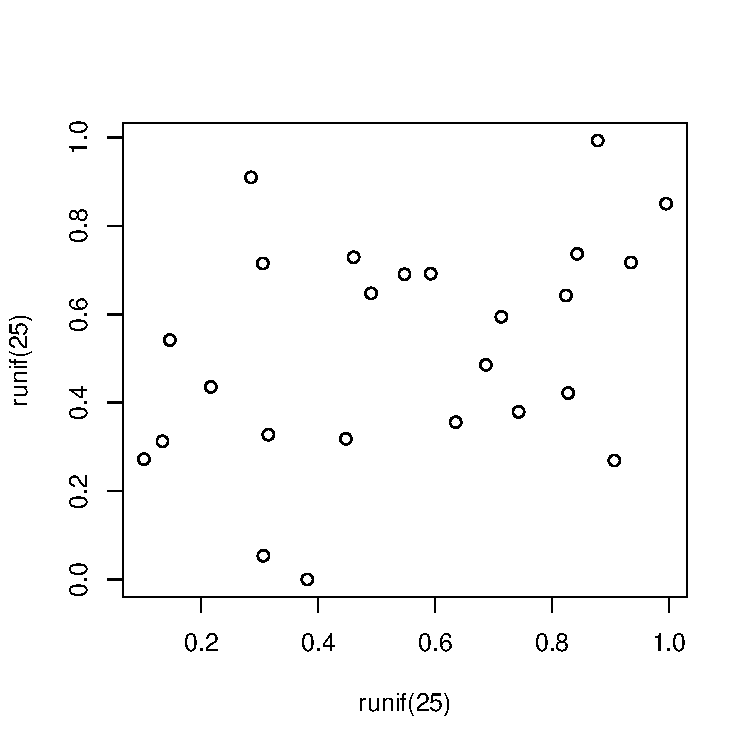
\includegraphics[width=0.5\linewidth]{Document_files/figure-latex/fig2-1} 

}

\caption{\label{fig2}A meaningless scatterplot.}\label{fig:fig2}
\end{figure}

\hypertarget{tables-coming-from-r}{%
\section{Tables coming from R}\label{tables-coming-from-r}}

Tables can also be generated using R chunks, as shown in Table
\ref{tab1} for example.

\begin{Shaded}
\begin{Highlighting}[]
\NormalTok{knitr}\SpecialCharTok{::}\FunctionTok{kable}\NormalTok{(}\FunctionTok{head}\NormalTok{(mtcars)[,}\DecValTok{1}\SpecialCharTok{:}\DecValTok{4}\NormalTok{], }
    \AttributeTok{caption =} \StringTok{"}\SpecialCharTok{\textbackslash{}\textbackslash{}}\StringTok{label\{tab1\}Caption centered above table"}
\NormalTok{)}
\end{Highlighting}
\end{Shaded}

\begin{longtable}[]{@{}lrrrr@{}}
\caption{\label{tab1}Caption centered above table}\tabularnewline
\toprule\noalign{}
& mpg & cyl & disp & hp \\
\midrule\noalign{}
\endfirsthead
\toprule\noalign{}
& mpg & cyl & disp & hp \\
\midrule\noalign{}
\endhead
\bottomrule\noalign{}
\endlastfoot
Mazda RX4 & 21.0 & 6 & 160 & 110 \\
Mazda RX4 Wag & 21.0 & 6 & 160 & 110 \\
Datsun 710 & 22.8 & 4 & 108 & 93 \\
Hornet 4 Drive & 21.4 & 6 & 258 & 110 \\
Hornet Sportabout & 18.7 & 8 & 360 & 175 \\
Valiant & 18.1 & 6 & 225 & 105 \\
\end{longtable}

\renewcommand\refname{References}
\bibliography{mybibfile.bib}


\end{document}
